\documentclass{article}
\usepackage{amsmath}
\usepackage{graphicx}
\usepackage{mathtools} % for Aboxed inside align


\graphicspath{{./images/}}

\title{Unit 2}
\author{Strannik}
\date{2023 June - 2023 July}


\begin{document}
\maketitle
\section{Vector Functions}
\begin{itemize}
  \item $x$, $y$ and $z$ are dependent variables in Parametric Equations
  \item $t$ is the parameter for some interval, $I$, on common domain, $k$
  \begin{align}
    \vec{r}(t) = \langle f(t), g(t), h(t) \rangle
  \end{align}
  \begin{itemize}
    \item \underline{You can only use common domain for $t$}
  \end{itemize}
  \item The terminal points of the vectors from a Vector Function create a curve through space (not a Surface) for the domain of $t$
  \item Sketching steps:
  \begin{enumerate}
    \item Identify $x$, $y$ and $z$
    \item Use 1 or more components to get a curve or a surface (get rid of $t$)
    \begin{itemize}
      \item For 2 components, sketch it on a plane
      \item For 3 components, the curve is on a surface
    \end{itemize}
  \item Use values of $t$ to find points and orientations
  \item Use values of $t$ that make one of components = 0
  \item Sometimes you can use more than 1 surface, but 1 is enough and you should choose the easiest
  \item The unused component gives you the curve \underline{on the surface}
  \end{enumerate}
\end{itemize}


\section{Derivatives of Vector Functions}
\begin{itemize}
  \item Tangent vector to a space curve or instantaneous velocity:
\begin{align}
  \vec{r}\,'(t) &= \lim_{\Delta t \to 0} \frac{\vec{r}(t + \Delta t) - \vec{r}(t)}{\Delta t} \\
  \vec{r}\,'(t) &= f'(t)\hat{i} + g'(t)\hat{j} + h'(t)\hat{k} 
\end{align}
  \item Dot Product and Cross Product derivatives are done simply by Product Rule
\end{itemize}


\section{Integrals of Vector Functions}
\begin{itemize}
  \item When evaluating integrals, $[F(t)]^b_a$, plug in $b$ and $a$ to each term in order to keep it organized
  \item Make 3 smaller integrals by separating the big integral's $\hat{i}, \hat{j}$ and $\hat{k}$ terms
  \item $+C$ is a constant vector
\end{itemize}


\section{Arc Length \& Parameterization}
\begin{align}
  L &= \int_{a}^{b} \sqrt{(f'(t))^2 + (g'(t))^2 + (h'(t))^2} \, dt \\
  L &= \int_{a}^{b} \|\vec{r}\,'(t)\| \, dt
\end{align}
\begin{itemize}
  \item $s(t)$ is the arc length function, while $L$ is just a number
  \begin{align}
    s(t) = \int_{a}^{t} \|\vec{r}\,'(u)\| \, du
  \end{align}
  \begin{itemize}
    \item $a$ is where $t$ begins
    \item Every $t$ is replaced by $u$
    \item Solve for $t$ and substitute this into given vector function to get $\vec{r}(s)$
  \end{itemize}
  \item Smooth curves can be reparameterized to:
  \begin{enumerate}
    \item "Walk the curve"
    \item Make some formulas easier
    \item \underline{$\vec{r}\,'(s)$ will always have magnitude of 1 (unit tangent vector)}
  \end{enumerate}
\end{itemize}


\section{TNB Frames (Frenet-Serret Frames)}
\begin{figure}[h]
  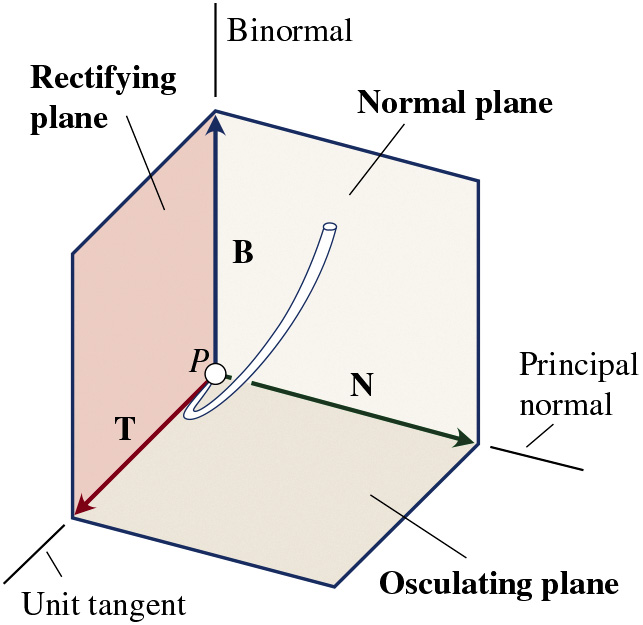
\includegraphics[scale=1]{TNB}
  \centering
  \label{fig:TNB}
\end{figure}
\begin{itemize}
  \item At every point, the TNB Frame gives unit vectors:
  \begin{enumerate}
    \item $\vec{T}$angent - derivative
    \begin{align}
      \vec{T}(s) &= \vec{r}\,'(s) \\
      \vec{T}(t) &= \frac{\vec{r}\,'(t)}{\|\vec{r}\,'(t)\|}
    \end{align}
    \item $\vec{N}$ormal - $\perp$ to tangent
    \begin{align}
      \vec{N}(t) = \frac{\vec{T}\,'(t)}{\|\vec{T}\,'(t)\|}
    \end{align}
    \begin{itemize}
      \item Vectors with constant magnitude are perpendicular to their derivatives: $\vec{v}\perp\vec{v}\,'$
    \end{itemize}
    \item $\vec{B}$inormal - mutually orthogonal to both
    \begin{align}
      \vec{B}(t) &= \vec{T}(t)\times\vec{N}(t) \\
      \vec{B}(t) &= \frac{\vec{r}\,'\times\vec{r}\,''}{\|\vec{r}\,'\times\vec{r}\,''\|}
    \end{align}
  \end{enumerate}
  \item \textbf{Curvature} is a measure of a curve's "failure to be a line", or how $\vec{T}$ is changing with respect to Arc Length
  \begin{align}
    \kappa &= \|\vec{T}\,'(s)\| \\
    \kappa &= \frac{\|\vec{T}\,'(t)\|}{\|\vec{r}\,'(t)\|} \\
    \kappa &= \frac{\|\vec{r}\,'(t)\times\vec{r}\,''(t)\|}{\|\vec{r}\,'(t)\|^3} \label{curvature-polynomials}
  \end{align}
  \begin{itemize}
    \item Use equation \ref{curvature-polynomials} if you need only curvature and your vector function consists of polynomials
  \end{itemize}
  \item \textbf{Torsion} is a measure of a curve's "failure to be contained in a plane"
  \begin{align}
    \tau &= \frac{(\vec{r}\,'\times\vec{r}\,'')\cdot\vec{r}\,'''}{\|\vec{r}\,'\times\vec{r}\,''\|^2} \label{torsion-polynomials} \\
    \tau &= -\frac{d\vec{B}}{ds}\cdot\vec{N}
  \end{align}
  \begin{itemize}
    \item Use equation \ref{torsion-polynomials} if you have vector function consisting of polynomials
  \end{itemize}
  \item \textbf{Osculating Circle}: at any point on a curve there will be a circle that fits that curve "best"
  \begin{itemize}
    \item The circle \underline{just} touches the curve ("kisses the curve")
    \item The curve and circle have the \underline{same tangent and curvature}
    \item The normal, which is the same for both circle and curve, points through circle's center
    \item The plane that contains the Osculating Circle, called the \textbf{Osculating Plane}, must contain $\vec{T}$ and $\vec{N}$, therefore $\vec{B}$ is its normal that can be used to describe it
    \item Osculating Circle's radius is called \textbf{Radius of Curvature}
    \begin{align}
      \rho = \frac{1}{\kappa}
    \end{align}
  \end{itemize}
  \item The \textbf{Normal Plane}, which contains $\vec{N}$ and $\vec{B}$, also contains \underline{all} vectors orthogonal to $\vec{T}$, so you can describe this plane with $\vec{T}$ as its normal
  \item You can convert regular functions into vector functions, which is called encapsulation:
  \begin{align}
    \begin{split}
      y &= f(x) \rightarrow \langle t, f(t), 0 \rangle \\
      x &= g(y) \rightarrow \langle g(t), t, 0 \rangle \\
      x &= f(t), \ y = g(t) \rightarrow \langle f(t), g(t), 0 \rangle \\
      r &= f(\theta) \rightarrow \langle f(t)\cos(t), f(t)\sin(t), 0 \rangle
    \end{split}
  \end{align}
\end{itemize}


\section{Velocity \& Acceleration}
\begin{itemize}
  \item For a vector function $\vec{r}(t)$:
  \begin{align}
    \begin{split}
      \vec{v}(t) &= \vec{r}\,'(t) \\
      \vec{a}(t) &= \vec{r}\,''(t) = \vec{v}\,'(t) \\
      v &= \|\vec{v}(t)\|
    \end{split}
  \end{align}
  \begin{itemize}
    \item $v$ is speed
  \end{itemize}
  \item Other acceleration equations:
  \begin{align}
    \begin{split}
      a_T &= v' = \frac{d}{dt}\|\vec{T}(t)\| \\
      a_N &= \kappa v^2 = \sqrt{\|\vec{a}\|^2 - (a_t)^2} \\
    \end{split} \\
    \vec{a} &= a_T\vec{T} + a_N\vec{N} \label{acceleration-TN-eq} \\
    \vec{a} &= \frac{\vec{r}\,'\cdot\vec{r}\,''}{\|\vec{r}\,'\|}\vec{T} + \frac{\|\vec{r}\,'\times\vec{r}\,''\|}{\|\vec{r}\,'\|}\vec{N} \\
  \end{align}
  \begin{itemize}
    \item $a_T$ in equation \ref{acceleration-TN-eq} is Tangent Component of Acceleration
    \item $a_N$ in equation \ref{acceleration-TN-eq} is Normal Component of Acceleration
  \end{itemize}
  \item Velocity and acceleration in polar coordinates:
  \begin{align}
    \vec{v} &= \dot{r}\vec{u}_r + r\dot{\theta}\vec{u}_\theta \\
    \vec{a} &= (\ddot{r} - r\dot{\theta}^2)\vec{u}_r + (r\ddot{\theta} + 2\dot{r}\dot{\theta})\vec{u}_\theta
  \end{align}
  \begin{itemize}
    \item The dots above letters are Newton's derivative notation
    \item Keep in mind that $\dot{r} = \frac{dr}{dt} = \frac{dr}{d\theta}\frac{d\theta}{dt}$ and $\ddot{r} = \frac{d}{dt}\dot{r} = \frac{d\dot{r}}{d\theta}\frac{d\theta}{dt}$
  \end{itemize}
  \item Projectile motion:
  \begin{align}
    \vec{r}(t) = (\vec{v}_0\cos(\alpha))t\hat{i} + \left( h + (\vec{v}_0\sin(\alpha))t - \frac{1}{2}gt^2 \right) \hat{j}
  \end{align}
  \begin{itemize}
    \item $\vec{v}_0$ is initial velocity (strange how it is a vector in the equation but in problems it is simply speed)
    \item $\alpha$ is angle of inclination
    \item $h$ is height
    \item $g$ is acceleration of gravity
  \end{itemize}
\end{itemize}
\end{document}
